\documentclass[9pt]{article}
\usepackage{amsmath,amssymb,amsthm,enumerate,tikz, subcaption, graphicx, hyperref}
\usetikzlibrary{matrix,arrows}


\addtolength{\evensidemargin}{-1.5in}
\addtolength{\oddsidemargin}{-1.5in}
\addtolength{\textwidth}{2in}
\addtolength{\textheight}{0.6in}
\addtolength{\topmargin}{-.2in}
\newcommand{\subjectTitle}{Data wrangling - Project Report}
\newcommand{\subjectDes}{The relationship between twitter usage and the occurence of
world events.}
\newcommand{\name}{James Zoryk.}
\newcommand{\SID}{$\:$2663347.}
\newcommand{\hw}{3}
\newcommand{\ddate}{06.10.2020}
%% If you want to define a new command, you can do it like this:

\title{\vspace{-130pt}
\huge \subjectTitle  \\ 
\vspace{10pt} \large \subjectDes 
\\ \vspace{10pt} \large \\ Group Members: \\
\begin{tabular}{c c c}
    James Zoryk & Sanne Petersen & Nicolina \\
    jzk340 & spn239 &id3 
\end{tabular}}
\date{}
\pagestyle{myheadings}
%%\markright{\name \SID \hfill Assignment \hw \hfill}



\begin{document}
\maketitle{}

\section{Research Question}
In this paper we shall investigate to see if there is any correlation between the density
of social media posts per a given time interval against discrete events in the news.
We hypothesis that a significant increase in the density for a giving time period shall
indicate either a notable news or world event that has occurred in that time period.
Furthermore, we believe that observing specific languages can lead to more localise
events. However, we note that many languages spread across different countries, thus the
phenomenon must be limited to localised languages.

The scope of work for this paper is to choose a significant social news event, and then
analysis the density of tweets created to see if we can observe a significant trend in
the data. For the purpose of this paper while shall observe a localise language, namely
Dutch. 

For this paper the social media posts that we shall consider will be `tweets` from the internet
server called twitter. The reason for this is that all the tweets are in public domain,
and that twitter serves as an online discussion platform, which is indicate by their
slogan \emph{"What’s happening"}. Also from a data point of view, each tweet contains a
lot of potential meta data that can be used. 

\end{enumerate}
\section{Data Source.}
A non-profit organisation called \emph{Archive Team}
(\href{https://wiki.archiveteam.org/}{\color{blue} \textbf{link}}) runs a web-scrapper that collects
data from all tweets created on the social media platform called twitter. This data is
collected into packets which can be
accessed by using the following website, from which the raw tweet data of a specific month
can be downloaded via a torrent, \href{
    https://archive.org/search?query=collection%3Atwitterstream}{\color{blue}
\textbf{here}}.


Since the data set mentioned above is rather dense as it contains more meta data than we
shall need for this investigation, a selection of reduce data sets have been produced and
can be accessed via our
\href{https://github.com/JamesZor/data-WranglingProject}{\color{blue} \textbf{GitHub}}
page, along with all other files related to this paper, including all figures.


\section{Data Wrangling methods}
\subsection{Getting the Data.}
Using the link provided in the Data Source part, the raw twitter data for the given can be
downloaded. This download file contains multiply \texttt{tar} files, which inside each
then contains approximately 1440 \texttt{gz} compressed \texttt{json} files. The
\texttt{json} files held more information than we required for this project, hence we need
to extract only the two following fields \emph{'created\_at'} and \emph{'lang'}, the first
giving us the
time the tweet was posted to the website and the second gives us information about the
user language it was written in. Note that twitter supports $34$ languages, with more
details can be found via
\href{https://developer.twitter.com/en/docs/twitter-for-websites/supported-languages}{\color{blue}
\textbf{twitter website}}.
In order to process all this downloaded information the python script
\texttt{TwitterZip2DataFrame.py} was created, which can be found via our
\href{https://github.com/JamesZor/data-WranglingProject/blob/main/TwitterZip2DataFrame.py}{\color{blue}\textbf{GitHub/TwitterZip2DataFrame}}.
Due to the sheer size of the files being process extra care is needed to process them.
Hence the python script unzips one of the tar files into a temporary file, from which a
multiprocess function is called to process the gz jsons files. 
This is to speed up the process. The json are convert in pandas data frames then the data frames
are stripped for the desired information, which are then concatenated with the other json
files and saved to the disk as csv files.  
Once all json files are proccessed in the .tar file, the temporary file is cleared to allow space 
for the next .tar file, until all are done. The result is that approximately 100Gb of raw twitter 
data can be filtered to under 7Gb of data, which is more user friendly. This processed
data can be found at
\href{https://github.com/JamesZor/data-WranglingProject/tree/main/dataSets/jan22All}{\color{blue}
\textbf{GitHub/Jan22All}}.

\subsection{Processing and visualising the data.}
The first task here is to get a better understanding of the data, in order to achieve this
we wish to plot all the data into a line plot, with time along the x-axis and the density
of tweets for the y-axis. Therefore we had to group all the tweet data into 1 hour bin of
posting their time, this was achieved by using pandas to convert the timeformat into
timestamp data types for the `created\_at' column and then using the pandas groupby function with specific options. The
result of which is we have a density of tweets per the hour. This data was plot by using
pandas line plot function, this can be seen in Figure [$\ref{fig:1a}$]. It become clear from the plot that the data contained outliers,
namely data points that contained less than the expected number of tweets for that time. There
are a number of reason for these outliers, such as the web-scrapper may not have been
working correctly for that time period or that the website twitter was down itself. Noting
that this would remove outliers below the line, while outliers above will be harder to
distinguish from real data. The
outliers in the data were removed, which resulted in a clear plot of the tweets, which can
be seen in Figure [$\ref{fig:1b}$]. Furthermore, using the pandas groupby function we can
split the data by the twitter supported language,
in our case we shall be looking at the Dutch tweets `nl'. Again removing outliers we can
generate a good plot for all Dutch tweets, see Figure [$\ref{fig:1c}$].
\begin{figure}[h!]
    \center
    \begin{subfigure}[b]{0.3\textwidth}
        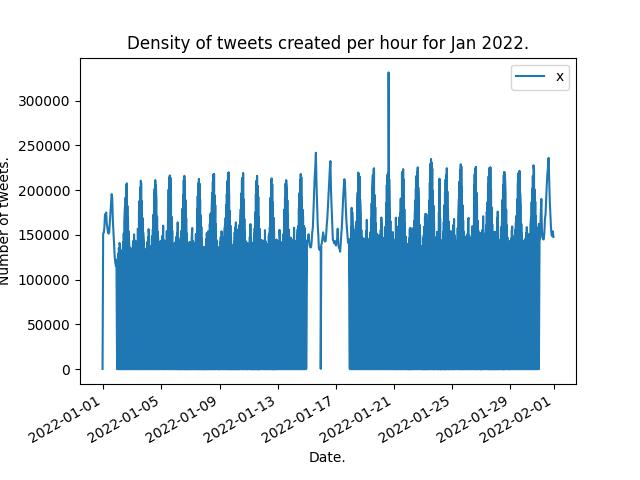
\includegraphics[width=\textwidth]{figures/JanAllraw.jpeg}
        \caption{Raw data.}
        \label{fig:1a}
    \end{subfigure}
    \begin{subfigure}[b]{0.3\textwidth}
        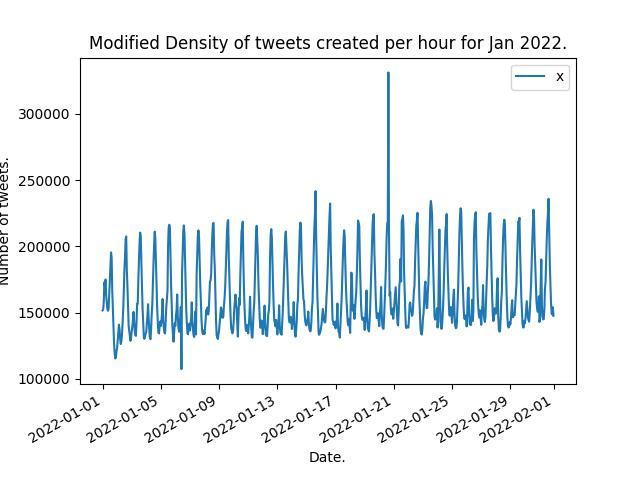
\includegraphics[scale=0.3]{figures/JanAllmod.jpeg}
        \caption{Outliers removed.}
        \label{fig:1b}
    \end{subfigure}
    \begin{subfigure}[b]{0.3\textwidth}
        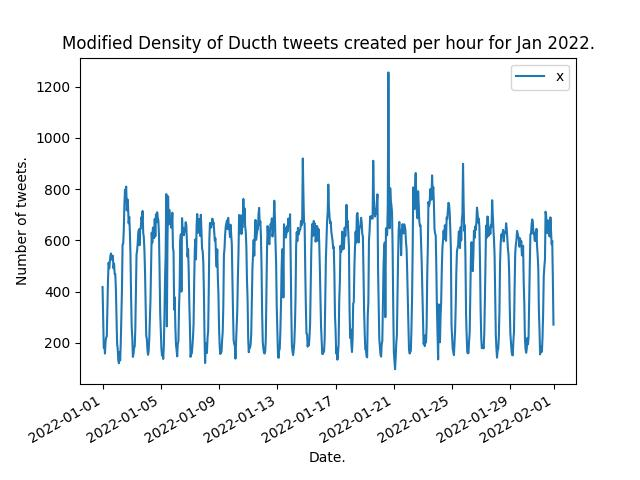
\includegraphics[scale=0.3]{figures/JanNLmod.jpeg}
        \caption{Dutch data, outliers removed.}
        \label{fig:1c}
    \end{subfigure}
    \caption{Line plots of density of tweets per 60min intervals.}
    \label{fig:g1}
\end{figure}

Since we are looking at discrete time events, we would like to have a better resolution of
the density of tweets per a time period. We achieve this by selecting again only the
Dutch tweets and then choosing a smaller time interval, in this case `2min`, while doing so
we also choose a smaller range of data, as we have indexed the dataframe by a Timestamp data
type, hence we can focus on the day 14-01-2022. Plotting this we see large fluctuations in the
data points, making the plot hard to read. The readability can be improved by using the
pandas rolling function in alignment with the mean function, the result is a smooth rolling
mean plot of the data, the results can be observed in Figure [$\ref{fig:2a}$].

As we want to test whether or not the behaviour of a specific day is in line with the
expected tweet density in general. Hence, we take 2min interval over a 24 hour period
again, which gives us 719 data points, then each day in the month is a column, thus each
cell indicates the density for that time interval. Using this data frame we can then
compute the mean and standard deviation of each time interval for the whole month. Noting
again we have large fluctuations, hence we then take a rolling mean of both the mean and
standard deviation in order to produce a smoother and more readable graph, see Figure
[$\ref{fig:2b}$]. We use the standard deviation in association with the plot function
fillbetween, which gives us a more visual indication of the confidence level of the data
points.

\begin{figure}[h!]
    \center
    \begin{subfigure}[b]{0.45\textwidth}
        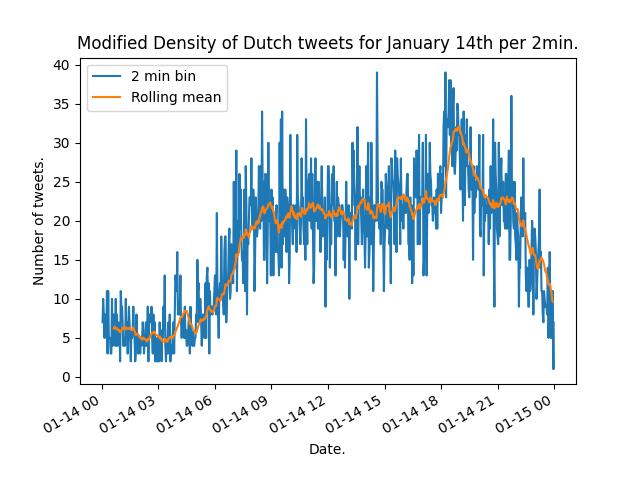
\includegraphics[scale=0.3]{figures/JanNLD14roll.jpeg}
        \caption{2min intervals, with rolling mean.} 
        \label{fig:2a}
    \end{subfigure}
    \begin{subfigure}[b]{0.45\textwidth}
        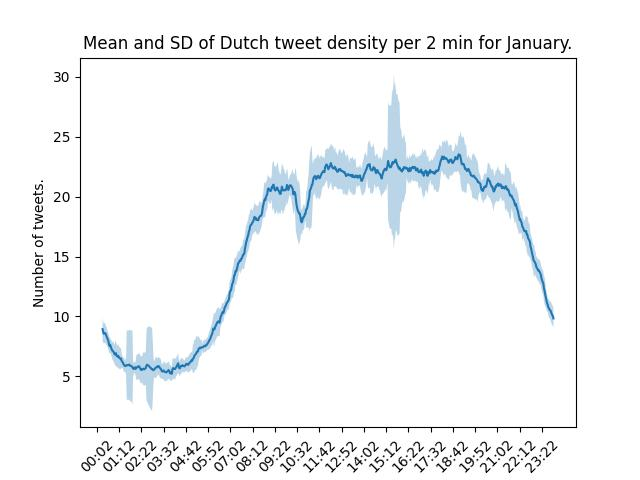
\includegraphics[scale=0.3]{figures/JanNLdayfill.jpeg}
        \caption{Rolling mean of the mean of each 2 min interval, with confidence itervals.} 
        \label{fig:2b}
    \end{subfigure}
    \caption{whats upppp.}
    \label{fig:2g}
\end{figure}

\section{Conclusion}

To test whether the hypothesis state in the open section of this paper has any merit, we
shall first consider a notable discrete social news event that occurred in January 2022,
namely the press conference held by the Dutch Health minister on January 14th at 19:00 and
also the related press conference on January 25th at 19:00, both at local time. The reason
for choosing these events is that it is a significant event that has the
impact to affect a lot of peoples lives, hence it will be a good topic for people to
discuss with each other. As a result we expecting to see an increase in the density of tweets,
however we are unsure when this will occur, in the build up, during or after the press
conference. Observe in Figure [$\ref{fig:3a}$] that we do indeed see peaks for both dates,
which both do look larger than the normal. To check this observation, we broke the day in
2min intervals, computed the mean and standard deviation for the month, and plotted both
the 14th and 25th against the rolling mean and $2\times SD$ interval, see Figure
[$\ref{fig:3b}$]. From Figure [$\ref{fig:3b}$], we see that both times the peak is well
above a $2\times SD$, which indicates this is not normal behaviour. Furthermore we note
that the press conference on the $14$th had a slightly larger reaction than the $25$th,
and in both cases it seems like the peak occur just before the events.  

\begin{figure}[h!]
    \center
    \begin{subfigure}[b]{0.45\textwidth}
        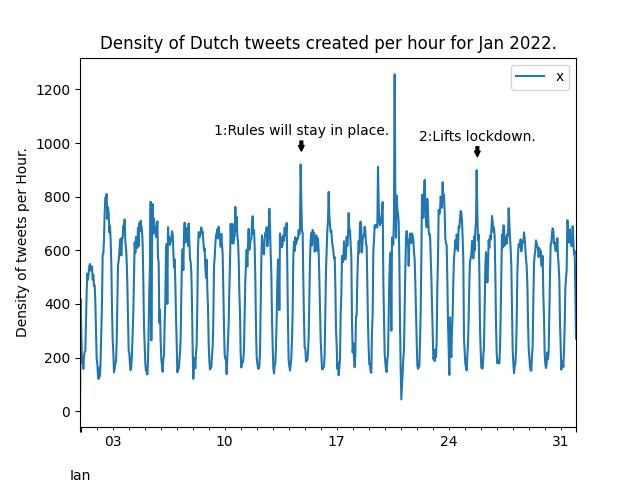
\includegraphics[scale=0.34]{figures/figNL60AnnoAX.jpeg}
        \caption{something.}
        \label{fig:3a}
    \end{subfigure}
    \begin{subfigure}[b]{0.45\textwidth}
        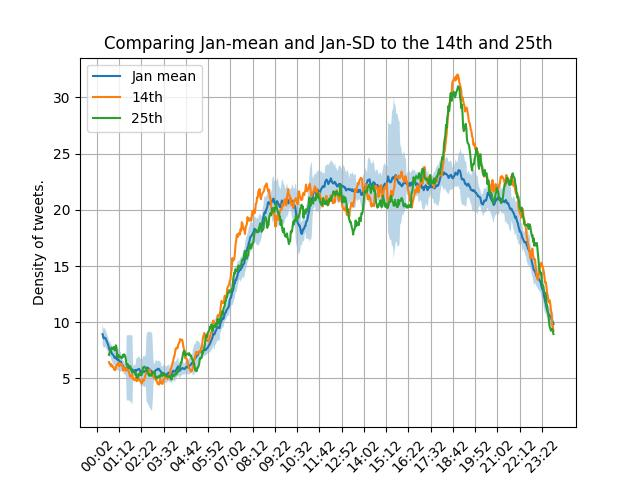
\includegraphics[scale=0.34]{figures/figNLComp.jpeg}
        \caption{something.}
        \label{fig:3b}
    \end{subfigure}
\end{figure}

Hence in our limited observation, we do see that there is a correlation between the
density of tweets created per time interval and world events. However we shall note the
limitation of these findings due to the small scale. The scope of this paper was limited
due to software, hardware and time, as processing the large amount of raw tweet data was a
significant issue thought this investigation. Thus further investigations into this topic
can perhaps research more world wide events, such as the eruption of Hunga Tonga-Hunga Ha'apai
volcano on 18th January 2022, which from our data we see a peak, Figure [$\ref{fig:1b}$].
One could investigate what event occur on around the 21st January 2022, as in both the
global and Dutch plot we see a large peak, however we were not successful at identify a
cause for this yet.






\end{document}
